\documentclass[natbib]{article}
\usepackage{microtype}
\usepackage{lmodern}
\usepackage{url}
\usepackage{xspace}
\usepackage{calc}
\usepackage{enumerate}
\usepackage{listings}
\usepackage{amsmath,amssymb}
\usepackage{rotating}
\usepackage{colortbl}
\usepackage{pifont}
\usepackage{tikz}
%\usetikzlibrary{shapes,shadows,arrows,calc,positioning,fit,matrix,mindmap,trees}
%\usepackage{pgfplots}
%\usepackage{pgfplotstable}
\usepackage{booktabs}
\usepackage{natbib}
\usepackage{colortbl}
\usepackage{algorithm2e}
% pantone colors

% More sensible defaults akin to \sloppy
% \tolerance 1414
% \hbadness 1414
% \emergencystretch 1.5em
% \hfuzz 0.3pt
% \widowpenalty=10000
% \clubpenalty=10000
% \vfuzz
% \hfuzz
% \raggedbottom

\newcommand{\ignore}[1]{}
\newcommand{\st}{\textit{s.\,t.}\xspace}
\newcommand{\eg}{\textit{e.\,g.}\xspace}
\newcommand{\ie}{\textit{i.\,e.}\xspace}
\newcommand{\cf}{\textit{cf.}\xspace}

\newcommand{\blackarrow}{{\color{black} \Pisymbol{pzd}{217}}}
\newcommand{\redarrow}{{\color{DarkRed} \Pisymbol{pzd}{217}}}
\newcommand{\minibox}[2]{\begin{minipage}{#1}\raggedright #2\end{minipage}}

\newcommand{\enquote}[1]{``#1''}

%\newcommand{\fixme}[1]{\begin{tikzpicture}
%\node[bottom color=red!80!white, top color=red!70!black, rounded corners,
%      font=\bf\color{white}\footnotesize] {
%  \begin{minipage}{.75\columnwidth}
%    FIXME\\
%    #1
%  \end{minipage}
%};
%\end{tikzpicture}
%}

\lstset{
  language=C,
  basicstyle=\small,%\scriptsize, %\footnotesize\ttfamily,
  keywordstyle={\bf},
  keywordstyle={[2]\it},%\color{Blue!40!black}},
  breaklines=true,
  identifierstyle=,
  stringstyle=\bf,
  commentstyle=\it\color{black!80},
  captionpos=b,
  numbers=left,
  stepnumber=3,
  columns=fullflexible
}

\begin{document}
\title{Typeforge}

\author{\small Markus Schordan, Nathan Pinnow}
%\end{tabular}
%\date{September 20, 2018}

\maketitle

\begin{abstract}
\noindent Typeforge is a tool for analysis and transformation of variable types in 
C/C++ programs. The main focus of development was to aid the development of 
mixed-precision programs through modification and searching of the AST. 
Typeforge does this through changing type information and inserting program 
instrumentation then outputting modified source code for the user or other tools to use.

\end{abstract}

\tableofcontents

%-------------------------------------------------------------------------

\section{Introduction}
\label{sec:intro}

Typeforge is based on the ROSE compiler infrastructure\footnote{\url{http://www.rosecompiler.org/}} 
and uses the ROSE abstract syntax tree as basis for its transformations. 
A main focus of Typeforge development was as part of a tool pipeline designed for 
the automatic generation of mixed-precision programs. For use in the pipeline 
Typeforge works with ADAPT~\cite{adapt} to insert the needed instrumentation to 
perform automatic differentiation for the purpose of finding variables error threshold.
Typeforge was also designed to work with CRAFT~\cite{CRAFT2013PARCO,CRAFT2013ICS,CRAFT2016} 
for the purpose of searching mixed-precision configurations built by Typeforge 
for the best performance.

\subsection{Handles}
Typeforge is capable of emitting string based handles for the purpose of variable identification. 
These handles are guaranteed to uniquely identify a variable in the program and can be used to 
specify a variable to Typeforge. The content of these handles is not guaranteed and is 
subject to change.

\section{Installation}

No additional configuration is required because Typeforge is configured as part of ROSE. Typeforge 
is not installed by default as part of ROSE, to install Typeforge after installing ROSE run 'make',
'make install', and optionally 'make check' in the \verb+projects/+ \verb+typeforge+ directory to 
install Typeforge. Typeforge is installed as 'typeforge' (at the same location as other ROSE tools, 
in the 'bin' directory of the ROSE installation).

\section{Command Line Options}
The command line options of Typeforge are parsed by Boost's program options 
library\footnote{\url{http://www.boost.org/doc/libs/1_63_0/doc/html/program_options.html}}.
The following command line options are listed when running \verb+typeforge --help+.
These main options below comprise general parameters such as spec file and explicit command line 
transformation. All filenames and unrecognized options will be passed directly to the ROSE compiler 
as command line options.

\begin{verbatim}
typeforge <filename> [OPTIONS]
Supported Options:
  -h [ --help ]                   Produce this help message.
  
  -v [ --version ]                Display the version of Typeforge.
  
  --compile                       Run backend compiler.
  
  --explicit                      Make all implicit casts explicit.
  
  --stats                         Print statistics on casts of built-in 
                                  floating point types.
                                  
  --trace                         Print program transformation operations 
                                  as they are performed.
\end{verbatim}
%set analysis may become hidden option
\begin{verbatim}
  --set-analysis                  Perform set analysis to determine which 
                                  variables must be changed together.
                                  
  --spec-file arg                 Name of Typeforge specification file.
  
  --csv-stats-file arg            Generate file [args] with transformation statistics.
  
  --float-var arg                 Change type of var [arg] to float.
  
  --double-var arg                Change type of var [arg] to double.
  
  --long-double-var arg           Change type of var [arg] to long double.
\end{verbatim}
\section{Specification File}
Typeforge uses a specification file for the user to specify what changes should be 
made to the source code. There are two formats supported for these files. a .json 
file and .tf file. The .json file is generated using ToolConfig and is intended 
for other programs to create specifications for Typeforge and the .tf file is a 
simplified version for developers to write manually. The .json format has a list 
of ToolActions stored in the actions field while the .tf file has one specification 
per line. Inside of ToolActions all fields are strings that describe the specification 
with the .tf file being the same fields without labels in a semi-colon separated list. 
The order in which specifications are written is not considered, if multiple 
specifications contradict the behavior is undefined. 

\subsection{Specifications}
For all specifications both specification file formats are shown. When double quotes 
are used it is to indicate that it is the literal string to use. For the JSON format 
all fields are in double quotes as they are input as a string type but the double quotes 
should not be used in the TF format.
\begin{enumerate}
\item{} Var Type Change -- This specification is for changing the type or base type 
of a specified variable. See section \ref{change} for more information on type changing. 
FunctionName can be either the name of the function where the variable is located or "\$global" 
for a global variable. VariableName can be the name of a single variable or a comma separated 
list of variables to change.
\begin{verbatim}
JSON Format:
action   = ("change_var_type" | "change_var_basetype")
scope    = FunctionName
name     = VariableName
to_type  = NewType

TF Format:
action;scope;name;to_type
\end{verbatim}

\item{} Handle Change -- This specification is to change a variables type based upon 
a compiler generated handle. For JSON providing a handle will override normal behavior 
and for .tf files a special command needs to be specified.

\begin{verbatim}
JSON Format:
action   = ("change_var_type" | "change_var_basetype")
handle   = CompilerHandle
to_type  = NewType

TF Format:
(change_handle_type | change_handle_basetype);handle;to_type
\end{verbatim}

\item{} Change Type -- This specification is to replace all variables of a type with a new type. 
VariableLocations is the locations where variables should be changed and has several forms. 
Use "\$global" to specify replacing globals, otherwise use function name followed by colon 
then parts of the function to change in a comma seperated list. Use args to change arguments, 
body to change the body of the function, and ret to change the return type. The function name 
can be replaced with * to change all functions. For example to change everything in main use 
"main:args,ret,body".

\begin{verbatim}
JSON Format:
action    = ("change_every_type" | "change_every_basetype")
scope     = VariableLocations
from_type = OldType
to_type   = NewType

TF Format:
action;scope;from_type=>to_type
\end{verbatim}

\item{} Listing Replacements -- Will output a list of possible replacements without 
changing the type. Will output a JSON file with the actions set so when input as a 
spec file will result in the changes being made. FileName is the file where the list will be 
written to, if it already exists the list will be appended to. SearchLocations can be the name 
of a function, "*" for all functions, "\$global" for just globals, or empty string for all. 
NewType is only used for writing a valid specification file to output.

\begin{verbatim}
action    = ("list_changes_type" | "list_changes_basetype")
scope     = SearchLocations
from_type = MatchType
to_type   = NewType
name      = FileName

TF Format:
action;scope;from_type;to_type;name
\end{verbatim}

\item{} Transformation -- Looks for patterns in the AST and will transform or insert 
code based upon the type of transformation. See section \ref{transform} for more 
information on transformations and transformation names. FunctionName can be and 
individual function name or "*" for all functions. MatchType semantics depends on 
the transformation.

\begin{verbatim}
JSON Format:
action    = "transform"
scope     = FunctionName 
from_type = MatchType
name      = TransformationName

TF Format:
action;scope;from_type;name
\end{verbatim}

\item{} Add Include -- Will add include to files in the AST. MatchFunction is used to specify 
only insert the include in files that define a specific function or use "*" for all files. 
IncludeFile is the name of the file to be included.

\begin{verbatim}
JSON Format:
action = "add_include"
scope  = MatchFunction
name   = IncludeFile

TF Format:
action;scope;name
\end{verbatim}

\item{} Pragma Replacement -- Will perform simple pragma replacement inside the AST. Will only 
replace pragmas that begin with MatchString excluding the \#pragma. Replace string is what the 
pragma will be replaced with. Can specify arguments by writing \$N where N is the argument 
number with 0 being the first token after the pragma in the source file including the matched string.
If using a .tf spec file the MatchString may not include semicolons but ReplaceString may 
use semicolons.

\begin{verbatim}
JSON Format:
action    = "replace_pragma"
from_type = MatchString
to_type   = ReplaceString

TF Format:
action;from_type;to_type
\end{verbatim}
\end{enumerate}

\subsection{Example Spec Files} \label{sec:expampleSpec}
This specification file is used as setup for the pipeline in section \ref{sec:pipeline}. 
Note there is a specification to change all doubles to AD\_real and a specification to 
list replacements for doubles. These can both work as they are performed on the original tree.
\begin{verbatim}
JSON Format:
{
  "version": "1",
  "tool_id": "Master",
  "actions": [
    {
      "action": "replace_pragma",
      "from_type": "adapt begin",
      "to_type": "AD_begin();"
    },
    {
      "action": "add_include",
      "name": "adapt-impl.cpp",
      "scope": "main"
    },
    {
      "action": "transform",
      "scope": "*",
      "from_type": "float",
      "name": "ad_intermediate_instrumentation"
    },
    {
      "action": "change_every_basetype",
      "scope": "*:args,ret,body",
      "from_type": "double",
      "to_type": "AD_real"
    },
    {
      "action": "list_changes_basetype",
      "scope": "",
      "from_type": "double",
      "to_type": "float",
      "name": "outputFile.json"
    }
  ]
}

TF Format:
replace_pragma;adapt begin;AD_begin();
add_include;main;adapt-impl.cpp
transform;*;float;ad_intermediate_instrumentation
change_every_basetype;*:args,ret,body;double=>AD_real
list_changes_basetype;;double;float;outputFile.json
\end{verbatim}
\vspace{5mm}
The next specification file is to change the type of two specific variables to float types.
One change is based upon the handle while the other is based upon specifying function 
name and variable name.

\begin{verbatim}
JSON Format:
{
  "version": "1",
  "tool_id": "CRAFT",
  "actions": [
  	{
  	  "action": "change_var_basetype",
  	  "handle": "Project<numbering,1>::FileList<numbering,1>::SourceFile
                  <name,/home/src/test.C>::VariableDeclaration<position,1.1-1.15>",
      "to_type": "float"
    }
    {
  	  "action": "change_var_basetype",
      "scope": "main",
      "to_type": "float",
      "name": "x"
    }
  ]
}

TF Format:
change_handle_basetype;Project<numbering,1>::FileList<numbering,1>::SourceFile
    <name,/home/src/test.C>::VariableDeclaration<position,1.1-1.15>;float
change_var_basetype;main;x;float
\end{verbatim}

\section{Type Change} \label{change}
All forms of changing a variables type will change the original declaration inside the AST 
as well as supporting base changing. If base is not specified the from type will be matched 
exactly regardless of pointers, arrays etc. If base is specified Typeforge will match based 
on types after stripping pointers, arrays, modifiers, reference, and typedefs. The type will 
be changed to a rebuilt type with the to type as the new base. For typedefs Typeforge will 
not create a new typedef, it will change the type to what the typedef represents with a 
new base type.

\section{Transformation} \label{transform}
\subsection{Array of Structure Access}
Can be done by specifying \verb+"name = arrayofstructs_access_transformation"+ to the transform 
specification.
\subsection{Hancock Access}
Can be done by specifying \verb+"name = readwrite_access_transformation"+ to the transform 
specification.
\subsection{ADAPT Instrumentation}
Can be done by specifying \verb+"name = ad_intermediate_instrumentation"+ to the transform 
specification, MatchType is not used. Will look for any location in the AST where a floating 
point type is assigned to or initialized then insert the correct AD\_intermidiate function 
call after the assignment with the name passed to ADAPT being set to the variables handle. 
If "\#pragma adapt begin" is included in the body will insert instrumentation for initialized 
globals immediately after the pragma. Will not do type replacement for AD\_real, including 
of ADAPT headers, or adapt pragma replacement.

\section{Analysis} \label{analysis}
\subsection{Variable Sets}
When changing the type of a variable it is possible that changing types will result in a 
compilation error due to interdependent variables. This happens when variables are connected, 
such as through assignment, and the types cannot simply be cast to be the same as with pointers 
or arrays. This results in every variable being part of a dependence set where all the variables 
in a given set must be changed together or the program will fail to compile. Given how these 
dependence sets are defined all variables will be part of a class and the classes will not intersect. 
Section \ref{sec:setAlg} shows the algorithm for set generation for just variables and 
section \ref{sec:setDef} shows a definition for the sets.

\subsubsection{Sets Algorithm} \label{sec:setAlg}
\begin{algorithm}[H]
\label{variableSetAlgo}
\SetAlgoLined
\KwResult{Dependence\_Sets}
Map$\langle$Node,Set$\langle$Node$\rangle\rangle$ Dependence\_Map;\\
List$\langle$Set$\langle$Node$\rangle\rangle$ Dependence\_Sets;\\
\For{All Variables}{
  Dependence\_Map.Add(Variable, Variable);
}
 \For{All AST Nodes}{
   \If{Node == Expression and Node.type == [Pointer or Array]}{
     \If{Node == Assignment}{
       Destination = Left  Hand Side;\\
       Origin       = Right Hand Side;\\
       \For{All Variable References in Origin}{
       Dependence\_Map.Add(VarRef, Destination);\\
       Dependence\_Map.Add(Destination, VarRef);
       }
     }
   }
 }
 \For{All Variable\_Set in Dependence\_Map}{
   Matched = Null;\\
   \For{All Set in Dependence\_Sets}{
     \If{Variable\_Set Intersects Set}{
       \eIf{Matched}{
         Matched.add(Set);\\
         Dependence\_Set.Remove(Set)
       }{
         Set.add(Variable\_Set);\\
         Matched = Set;
       }
     }
   }
   \If{Not Matched}{
     Dependence\_Sets.Add(Variable\_Set)
   }
 }
 \caption{Algorithm for building variable sets}
\end{algorithm}
\subsubsection{Sets Definition} \label{sec:setDef}
\begin{gather} 
V = \text{Set of all variables, function parameters, and function return.}\\
M = \text{Set of variable sets. Each Variable Links to a single set.}\\
S = \text{Final set of interdependent sets}\\
\forall i \in V(\exists! j \in S(i \in j))\\
\forall x \in M(\exists! y \in S(x \cap y \neq \emptyset) \wedge 
\exists! z \in S(x \subseteq z))
\end{gather}
\section{Use Cases}
\subsection{CRAFT-ADAPT Pipeline}\label{sec:pipeline}
%\begin{figure}[h]
%    \centering
%    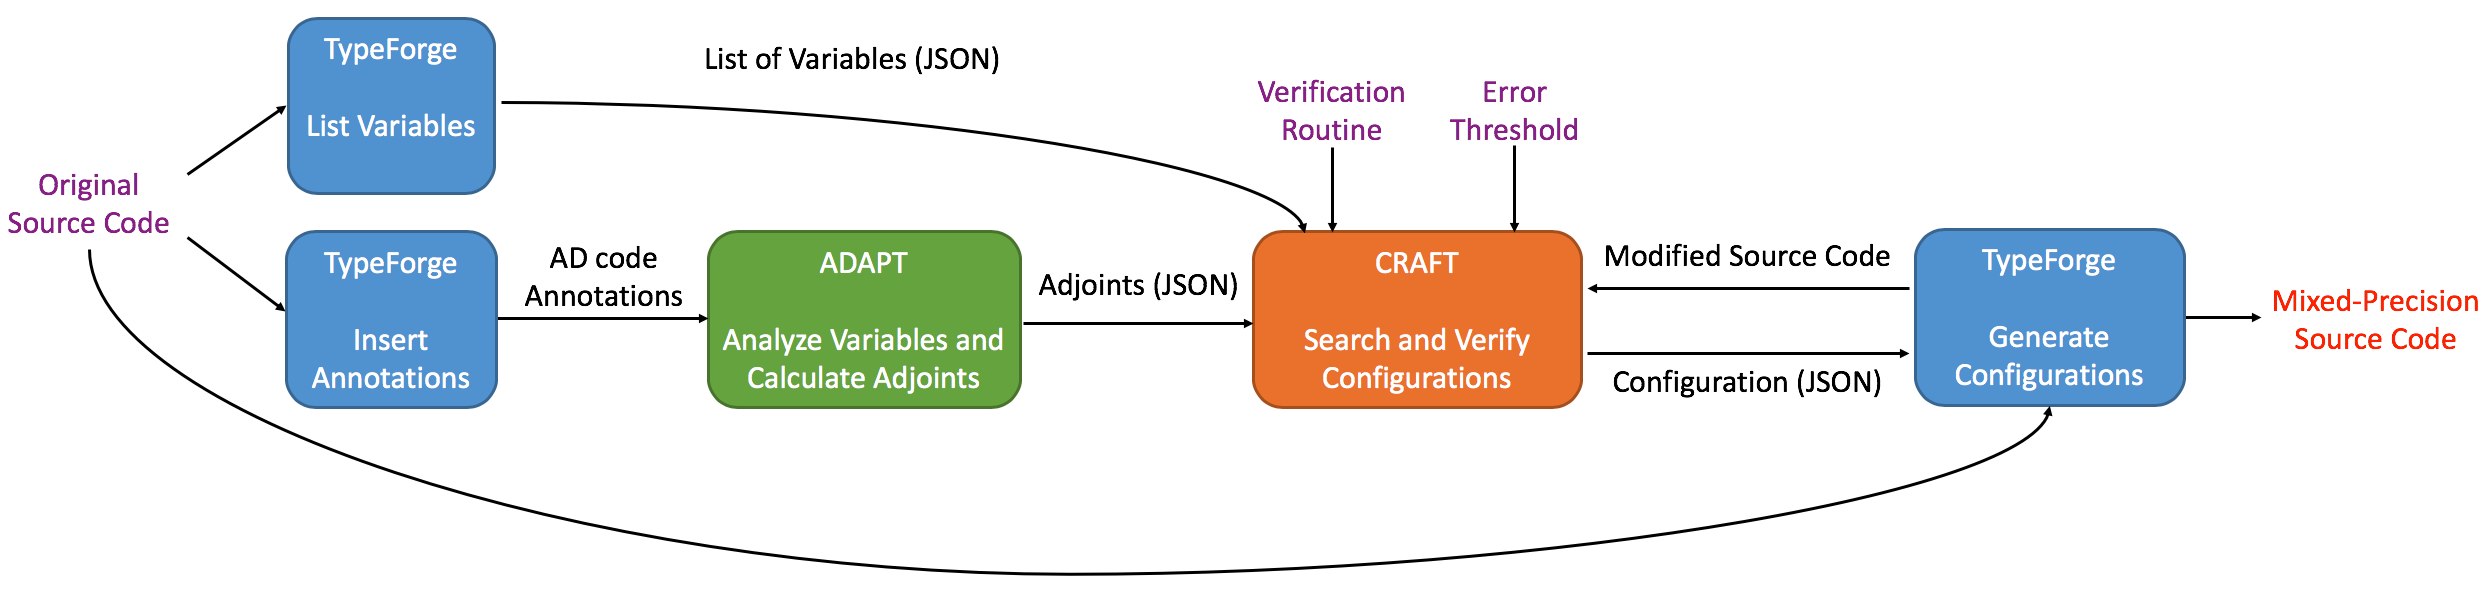
\includegraphics[width=\textwidth]{pipeline.png}
%    \caption{\textsf{Diagram of pipeline structure}}
%    \label{fig:pipeline}
%\end{figure}
\noindent
Typeforge has several uses in the pipeline for automatic generation of mixed precision programs.
%as seen in figure \ref{fig:pipeline}. 
In order for craft to conduct a proper search it needs to define 
a search space which can be done by Typeforge by looking for all declarations in the AST. This 
list can be refined by looking at sets to avoid searching configurations that will not compile. 
When CRAFT tests a configuration it passes the appropriate specification file to Typeforge so 
that it can generate new source code and compile the configuration. This lets CRAFT gain 
performance metrics on a configuration instead of estimations. To refine the search space ADAPT 
feeds precision information to CRAFT but for ADAPT to run modifications need to be made to the 
source code. These modifications are pragma replacement, adding includes, replacing floating point 
types with AD\_real, and adding ADAPT function calls. All of the ADAPT modifications and Variable 
listing can be done with Typeforge with a single specification shown in section \ref{sec:expampleSpec}.
\bibliographystyle{plain}
\bibliography{typeforge}

\end{document}

